% Generated by Sphinx.
\def\sphinxdocclass{report}
\documentclass[letterpaper,10pt,english]{sphinxmanual}
\usepackage[utf8]{inputenc}
\DeclareUnicodeCharacter{00A0}{\nobreakspace}
\usepackage[T1]{fontenc}
\usepackage[english]{babel}
\usepackage{times}
\usepackage[Sonny]{fncychap}
\usepackage{longtable}
\usepackage{sphinx}
\usepackage{multirow}


\title{EARSmilter Documentation}
\date{September 07, 2012}
\release{1.0}
\author{Larry G. Wapnitsky}
\newcommand{\sphinxlogo}{
\includegraphics{earslogo.png}\par}
\renewcommand{\releasename}{Release}
\makeindex

\makeatletter
\def\PYG@reset{\let\PYG@it=\relax \let\PYG@bf=\relax%
    \let\PYG@ul=\relax \let\PYG@tc=\relax%
    \let\PYG@bc=\relax \let\PYG@ff=\relax}
\def\PYG@tok#1{\csname PYG@tok@#1\endcsname}
\def\PYG@toks#1+{\ifx\relax#1\empty\else%
    \PYG@tok{#1}\expandafter\PYG@toks\fi}
\def\PYG@do#1{\PYG@bc{\PYG@tc{\PYG@ul{%
    \PYG@it{\PYG@bf{\PYG@ff{#1}}}}}}}
\def\PYG#1#2{\PYG@reset\PYG@toks#1+\relax+\PYG@do{#2}}

\expandafter\def\csname PYG@tok@gd\endcsname{\def\PYG@tc##1{\textcolor[rgb]{0.63,0.00,0.00}{##1}}}
\expandafter\def\csname PYG@tok@gu\endcsname{\let\PYG@bf=\textbf\def\PYG@tc##1{\textcolor[rgb]{0.50,0.00,0.50}{##1}}}
\expandafter\def\csname PYG@tok@gt\endcsname{\def\PYG@tc##1{\textcolor[rgb]{0.00,0.25,0.82}{##1}}}
\expandafter\def\csname PYG@tok@gs\endcsname{\let\PYG@bf=\textbf}
\expandafter\def\csname PYG@tok@gr\endcsname{\def\PYG@tc##1{\textcolor[rgb]{1.00,0.00,0.00}{##1}}}
\expandafter\def\csname PYG@tok@cm\endcsname{\let\PYG@it=\textit\def\PYG@tc##1{\textcolor[rgb]{0.25,0.50,0.56}{##1}}}
\expandafter\def\csname PYG@tok@vg\endcsname{\def\PYG@tc##1{\textcolor[rgb]{0.73,0.38,0.84}{##1}}}
\expandafter\def\csname PYG@tok@m\endcsname{\def\PYG@tc##1{\textcolor[rgb]{0.13,0.50,0.31}{##1}}}
\expandafter\def\csname PYG@tok@mh\endcsname{\def\PYG@tc##1{\textcolor[rgb]{0.13,0.50,0.31}{##1}}}
\expandafter\def\csname PYG@tok@cs\endcsname{\def\PYG@tc##1{\textcolor[rgb]{0.25,0.50,0.56}{##1}}\def\PYG@bc##1{\setlength{\fboxsep}{0pt}\colorbox[rgb]{1.00,0.94,0.94}{\strut ##1}}}
\expandafter\def\csname PYG@tok@ge\endcsname{\let\PYG@it=\textit}
\expandafter\def\csname PYG@tok@vc\endcsname{\def\PYG@tc##1{\textcolor[rgb]{0.73,0.38,0.84}{##1}}}
\expandafter\def\csname PYG@tok@il\endcsname{\def\PYG@tc##1{\textcolor[rgb]{0.13,0.50,0.31}{##1}}}
\expandafter\def\csname PYG@tok@go\endcsname{\def\PYG@tc##1{\textcolor[rgb]{0.19,0.19,0.19}{##1}}}
\expandafter\def\csname PYG@tok@cp\endcsname{\def\PYG@tc##1{\textcolor[rgb]{0.00,0.44,0.13}{##1}}}
\expandafter\def\csname PYG@tok@gi\endcsname{\def\PYG@tc##1{\textcolor[rgb]{0.00,0.63,0.00}{##1}}}
\expandafter\def\csname PYG@tok@gh\endcsname{\let\PYG@bf=\textbf\def\PYG@tc##1{\textcolor[rgb]{0.00,0.00,0.50}{##1}}}
\expandafter\def\csname PYG@tok@ni\endcsname{\let\PYG@bf=\textbf\def\PYG@tc##1{\textcolor[rgb]{0.84,0.33,0.22}{##1}}}
\expandafter\def\csname PYG@tok@nl\endcsname{\let\PYG@bf=\textbf\def\PYG@tc##1{\textcolor[rgb]{0.00,0.13,0.44}{##1}}}
\expandafter\def\csname PYG@tok@nn\endcsname{\let\PYG@bf=\textbf\def\PYG@tc##1{\textcolor[rgb]{0.05,0.52,0.71}{##1}}}
\expandafter\def\csname PYG@tok@no\endcsname{\def\PYG@tc##1{\textcolor[rgb]{0.38,0.68,0.84}{##1}}}
\expandafter\def\csname PYG@tok@na\endcsname{\def\PYG@tc##1{\textcolor[rgb]{0.25,0.44,0.63}{##1}}}
\expandafter\def\csname PYG@tok@nb\endcsname{\def\PYG@tc##1{\textcolor[rgb]{0.00,0.44,0.13}{##1}}}
\expandafter\def\csname PYG@tok@nc\endcsname{\let\PYG@bf=\textbf\def\PYG@tc##1{\textcolor[rgb]{0.05,0.52,0.71}{##1}}}
\expandafter\def\csname PYG@tok@nd\endcsname{\let\PYG@bf=\textbf\def\PYG@tc##1{\textcolor[rgb]{0.33,0.33,0.33}{##1}}}
\expandafter\def\csname PYG@tok@ne\endcsname{\def\PYG@tc##1{\textcolor[rgb]{0.00,0.44,0.13}{##1}}}
\expandafter\def\csname PYG@tok@nf\endcsname{\def\PYG@tc##1{\textcolor[rgb]{0.02,0.16,0.49}{##1}}}
\expandafter\def\csname PYG@tok@si\endcsname{\let\PYG@it=\textit\def\PYG@tc##1{\textcolor[rgb]{0.44,0.63,0.82}{##1}}}
\expandafter\def\csname PYG@tok@s2\endcsname{\def\PYG@tc##1{\textcolor[rgb]{0.25,0.44,0.63}{##1}}}
\expandafter\def\csname PYG@tok@vi\endcsname{\def\PYG@tc##1{\textcolor[rgb]{0.73,0.38,0.84}{##1}}}
\expandafter\def\csname PYG@tok@nt\endcsname{\let\PYG@bf=\textbf\def\PYG@tc##1{\textcolor[rgb]{0.02,0.16,0.45}{##1}}}
\expandafter\def\csname PYG@tok@nv\endcsname{\def\PYG@tc##1{\textcolor[rgb]{0.73,0.38,0.84}{##1}}}
\expandafter\def\csname PYG@tok@s1\endcsname{\def\PYG@tc##1{\textcolor[rgb]{0.25,0.44,0.63}{##1}}}
\expandafter\def\csname PYG@tok@gp\endcsname{\let\PYG@bf=\textbf\def\PYG@tc##1{\textcolor[rgb]{0.78,0.36,0.04}{##1}}}
\expandafter\def\csname PYG@tok@sh\endcsname{\def\PYG@tc##1{\textcolor[rgb]{0.25,0.44,0.63}{##1}}}
\expandafter\def\csname PYG@tok@ow\endcsname{\let\PYG@bf=\textbf\def\PYG@tc##1{\textcolor[rgb]{0.00,0.44,0.13}{##1}}}
\expandafter\def\csname PYG@tok@sx\endcsname{\def\PYG@tc##1{\textcolor[rgb]{0.78,0.36,0.04}{##1}}}
\expandafter\def\csname PYG@tok@bp\endcsname{\def\PYG@tc##1{\textcolor[rgb]{0.00,0.44,0.13}{##1}}}
\expandafter\def\csname PYG@tok@c1\endcsname{\let\PYG@it=\textit\def\PYG@tc##1{\textcolor[rgb]{0.25,0.50,0.56}{##1}}}
\expandafter\def\csname PYG@tok@kc\endcsname{\let\PYG@bf=\textbf\def\PYG@tc##1{\textcolor[rgb]{0.00,0.44,0.13}{##1}}}
\expandafter\def\csname PYG@tok@c\endcsname{\let\PYG@it=\textit\def\PYG@tc##1{\textcolor[rgb]{0.25,0.50,0.56}{##1}}}
\expandafter\def\csname PYG@tok@mf\endcsname{\def\PYG@tc##1{\textcolor[rgb]{0.13,0.50,0.31}{##1}}}
\expandafter\def\csname PYG@tok@err\endcsname{\def\PYG@bc##1{\setlength{\fboxsep}{0pt}\fcolorbox[rgb]{1.00,0.00,0.00}{1,1,1}{\strut ##1}}}
\expandafter\def\csname PYG@tok@kd\endcsname{\let\PYG@bf=\textbf\def\PYG@tc##1{\textcolor[rgb]{0.00,0.44,0.13}{##1}}}
\expandafter\def\csname PYG@tok@ss\endcsname{\def\PYG@tc##1{\textcolor[rgb]{0.32,0.47,0.09}{##1}}}
\expandafter\def\csname PYG@tok@sr\endcsname{\def\PYG@tc##1{\textcolor[rgb]{0.14,0.33,0.53}{##1}}}
\expandafter\def\csname PYG@tok@mo\endcsname{\def\PYG@tc##1{\textcolor[rgb]{0.13,0.50,0.31}{##1}}}
\expandafter\def\csname PYG@tok@mi\endcsname{\def\PYG@tc##1{\textcolor[rgb]{0.13,0.50,0.31}{##1}}}
\expandafter\def\csname PYG@tok@kn\endcsname{\let\PYG@bf=\textbf\def\PYG@tc##1{\textcolor[rgb]{0.00,0.44,0.13}{##1}}}
\expandafter\def\csname PYG@tok@o\endcsname{\def\PYG@tc##1{\textcolor[rgb]{0.40,0.40,0.40}{##1}}}
\expandafter\def\csname PYG@tok@kr\endcsname{\let\PYG@bf=\textbf\def\PYG@tc##1{\textcolor[rgb]{0.00,0.44,0.13}{##1}}}
\expandafter\def\csname PYG@tok@s\endcsname{\def\PYG@tc##1{\textcolor[rgb]{0.25,0.44,0.63}{##1}}}
\expandafter\def\csname PYG@tok@kp\endcsname{\def\PYG@tc##1{\textcolor[rgb]{0.00,0.44,0.13}{##1}}}
\expandafter\def\csname PYG@tok@w\endcsname{\def\PYG@tc##1{\textcolor[rgb]{0.73,0.73,0.73}{##1}}}
\expandafter\def\csname PYG@tok@kt\endcsname{\def\PYG@tc##1{\textcolor[rgb]{0.56,0.13,0.00}{##1}}}
\expandafter\def\csname PYG@tok@sc\endcsname{\def\PYG@tc##1{\textcolor[rgb]{0.25,0.44,0.63}{##1}}}
\expandafter\def\csname PYG@tok@sb\endcsname{\def\PYG@tc##1{\textcolor[rgb]{0.25,0.44,0.63}{##1}}}
\expandafter\def\csname PYG@tok@k\endcsname{\let\PYG@bf=\textbf\def\PYG@tc##1{\textcolor[rgb]{0.00,0.44,0.13}{##1}}}
\expandafter\def\csname PYG@tok@se\endcsname{\let\PYG@bf=\textbf\def\PYG@tc##1{\textcolor[rgb]{0.25,0.44,0.63}{##1}}}
\expandafter\def\csname PYG@tok@sd\endcsname{\let\PYG@it=\textit\def\PYG@tc##1{\textcolor[rgb]{0.25,0.44,0.63}{##1}}}

\def\PYGZbs{\char`\\}
\def\PYGZus{\char`\_}
\def\PYGZob{\char`\{}
\def\PYGZcb{\char`\}}
\def\PYGZca{\char`\^}
\def\PYGZam{\char`\&}
\def\PYGZlt{\char`\<}
\def\PYGZgt{\char`\>}
\def\PYGZsh{\char`\#}
\def\PYGZpc{\char`\%}
\def\PYGZdl{\char`\$}
\def\PYGZti{\char`\~}
% for compatibility with earlier versions
\def\PYGZat{@}
\def\PYGZlb{[}
\def\PYGZrb{]}
\makeatother

\begin{document}

\maketitle
\tableofcontents
\phantomsection\label{index::doc}



\chapter{What is the EARS Milter?}
\label{about:wrt-e-mail-attachment-removal-retrieval-system-ears-milter}\label{about::doc}\label{about:what-is-the-ears-milter}
While wonderfully convenient, receiving files from clients and consultants through email has its drawbacks.

First there’s the mailbox bloat. One 8MB email and wham!, your mailbox is full and you can’t send.
Then there’s the PST file size limit to contend with.
And if you need bigger files? Forgetaboutit!
FTP? SendIT? There are ways around using email to receive files but the best of them aren’t half as simple.
Can’t we just….? Now, we can!

Introducing the \emph{Email Attachment Removal/Retrieval System (EARS)}. Email
attachment magic – automatically. Now, if someone outside the office sends you
an email that exceeds a set threshold in size (currently 8MB), instead of being
rejected, the message is passed to the Email Attachment Removal/Retrieval
System. EARS saves any attachments larger than 160K to a temporary storage
location, removes them from the email message and creates a new attachment
named ‘Retrieve\_Attachments.html’ before passing it on to your mailbox. The
result is that you receive a nice small email with links to the original
attachments that you can download and save to the location of your choice. You
can even retrieve the attachments using your iPhone/iPad \footnote{
iPhone/iPad compatibility is limited to files that are readable on your device based on installed apps.
} or Outlook Web
Access!

Incoming Email attachment size is no longer limited by WRT, only by the sender’s email system.

Here’s what it looks like:

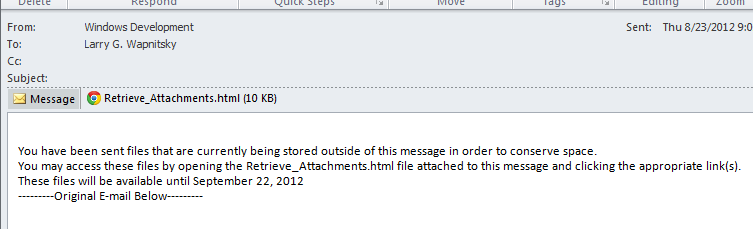
\includegraphics{EARSmilter.png}

Notice the subject line has been appended with “{[}Attachments Processed{]}”. This tells you that the message was passed to the EARS system and attachments have been saved and removed. Also notice the ‘Retrieve\_Attachments.html’ attachment – this is where you get your files back when you open it.

Open the ‘Retrieve\_Attachments.html’ by double-clicking in Outlook and the page will open in your browser. Use the links to save your files to the location of your choice. But do it right away because the files will be deleted permanently (and un-retrievably) from the temporary location 30 days after the message was received whether you’ve saved them or not!

EARS was conceived of by your IT team in response to direct feedback from you and was created by our one and only Larry Wapnitsky using FREE open-source software. No dollars were harmed during its development.


\chapter{EARS Milter Requirements}
\label{requirements:ears-milter-requirements}\label{requirements::doc}
The EARS Milter is a Python-based \href{http://www.milter.org}{mail-filter} written for the \href{http://www.postfix.org}{postfix} and \href{http://www.sendmail.com/sm/open\_source/docs/}{sendmail} mail transfer agents (MTAs).

\begin{notice}{note}{Note:}
\emph{Postfix} or \emph{sendmail} must be installed on your system in order for this milter to function properly.
It may work with any other MTA that supports milters but has only been tested with postfix and sendmail.
\end{notice}

\begin{notice}{note}{Note:}
\emph{This milter has only been tested on Python 2.7 running on Debian Squeeze/Wheezy}
\end{notice}


\section{Server Requirements}
\label{requirements:server-requirements}
The following software is required for the Milter to run:
\begin{itemize}
\item {} 
\href{http://www.debian.org/releases}{Debian Squeeze/Wheezy}

\item {} 
\href{http://www.mysql.com}{MySQL database}

\item {} 
\href{http://projects.apache.org/projects/http\_server.html}{Apache HTTP Server}

\item {} 
\href{http://www.php.net}{PHP 5.x}

\item {} 
\href{http://www.postfix.org}{postfix} or \href{http://www.sendmail.com/sm/open\_source/docs/}{sendmail}

\item {} 
\href{http://git-scm.com}{Git} - required to download the Milter from the development repository

\item {} 
cifs-utils

\end{itemize}


\section{Python Requirements}
\label{requirements:python-requirements}
The following Python modules are required on the system in order for the EARS Milter to function:
\begin{itemize}
\item {} 
\href{http://python.org}{Python 2.7}

\item {} 
\href{http://sqlalchemy.org}{SQLAlchemy}

\item {} 
\href{http://www.bmsi.com/python/milter.html}{pymilter}

\item {} 
\href{http://mysql-python.sourceforge.net/MySQLdb.html}{MySQLdb}

\item {} 
\href{https://github.com/koodaamo/tnefparse}{tnefparse}

\item {} 
\href{http://www.makotemplates.org/}{mako}

\end{itemize}


\section{Recommended Software}
\label{requirements:recommended-software}
While not necessary, this software should be installed as it will be referenced during the installation procedure:
\begin{itemize}
\item {} 
telnet

\item {} 
rsyslog

\item {} 
logrotate

\item {} 
\href{http://www.webmin.com/deb.html}{Webmin}

\end{itemize}


\section{Optional Software}
\label{requirements:optional-software}
The following software is optional, but is useful for diagnostics
\begin{itemize}
\item {} 
\href{http://www.phpmyadmin.net}{phpMyAdmin}

\end{itemize}


\chapter{EARS Milter Installation}
\label{installation:ears-milter-installation}\label{installation::doc}\label{installation:id1}\setbox0\vbox{
\begin{minipage}{0.95\linewidth}
\begin{itemize}
\item {} 
{\hyperref[installation:server-installation]{Server Installation}}
\begin{itemize}
\item {} 
{\hyperref[installation:debian-install]{Debian Install}}

\item {} 
{\hyperref[installation:web-server-installation]{Web Server Installation}}

\item {} 
{\hyperref[installation:git-installation]{Git Installation}}

\item {} 
{\hyperref[installation:mail-server-installation]{Mail Server Installation}}
\begin{itemize}
\item {} 
{\hyperref[installation:postfix-option-1]{Postfix (Option 1)}}

\item {} 
{\hyperref[installation:sendmail-option-2]{Sendmail (Option 2)}}

\end{itemize}

\end{itemize}

\item {} 
{\hyperref[installation:python-installation-configuration]{Python Installation/Configuration}}
\begin{itemize}
\item {} 
{\hyperref[installation:the-python-method-preferred]{The Python Method (preferred)}}

\item {} 
{\hyperref[installation:the-debian-method]{The Debian Method}}

\end{itemize}

\item {} 
{\hyperref[installation:optional-software-installation]{Optional Software Installation}}
\begin{itemize}
\item {} 
{\hyperref[installation:phpmyadmin]{phpMyAdmin}}

\item {} 
{\hyperref[installation:webmin-installation]{Webmin Installation}}

\end{itemize}

\item {} 
{\hyperref[installation:accquiring-and-configuring-the-milter]{Accquiring and configuring the Milter}}

\end{itemize}
\end{minipage}}
\begin{center}\setlength{\fboxsep}{5pt}\shadowbox{\box0}\end{center}


\section{Server Installation}
\label{installation:server-installation}
This milter has been tested on Debian Squeeze/Wheezy using a LAMP
(Linux/Apache/MySQL/PHP)-based web server \footnote{
Adapted from HowtoForge's \href{http://www.howtoforge.com/installing-apache2-with-php5-and-mysql-support-on-debian-squeeze-lamp}{Installing Apache2 With PHP5 And MySQL Support On Debian Squeeze (LAMP)}
}.


\subsection{Debian Install}
\label{installation:debian-install}
Installing a Debian Squeeze/Wheezy server is a fairly straight-forward
procedure.  The best method to use can be found via HowtoForge's
\href{http://www.howtoforge.com/perfect-server-debian-squeeze-ispconfig-2}{The Perfect Server - Debian Squeeze (Debian 6.0) {[}ISPConfig 2{]}} and following
it up through \textbf{8 Change The Default Shell} on page 3.

\begin{notice}{note}{Note:}
In WRT's environment, virtual linux servers are set up using Linux Containers (\href{http://lxc.sourceforge.net/}{lxc}).

To create a new system, log in to the LXC server as root and use the  \code{lxc-prepare} \href{http://www.google.com/url?sa=t\&rct=j\&q=\&esrc=s\&source=web\&cd=1\&ved=0CCAQFjAA\&url=http://mindref.blogspot.com/2011/01/debian-lxc-create.html\&ei=Gxk-UO7IMIH86wGEoIGgDg\&usg=AFQjCNH8nf1DFSRpLmQigOgj8AsU-xhA3Q\&sig2=KpSOTudr5eTp97MCE7aLRw}{script}.

Make sure to edit \code{/var/lib/lxc/\textless{}machine name\textgreater{}/rootfs/etc/network/interfaces} and enter the appropriate
static IP, routing and gateway information.
\end{notice}

After logging in, make sure to install \code{anacron}, \code{cifs-utils}, \code{telnet},
\code{rsyslog} and \code{logrotate}.

\begin{Verbatim}[commandchars=\\\{\},formatcom=\footnotesize]
aptitude install telnet rsyslog logrotate cifs-utils anacron
\end{Verbatim}


\subsection{Web Server Installation}
\label{installation:web-server-installation}
\begin{notice}{note}{Note:}
Unless otherwise specified, all commands are run as the \code{root} user.
\end{notice}

The web server needs to be set up in a LAMP configuration (Apache Web Server,
MySQL, PHP)
\begin{enumerate}
\item {} 
Install MySQL

\begin{Verbatim}[commandchars=\\\{\},formatcom=\footnotesize]
\PYGZpc{} aptitude install mysql-server mysql-client
\end{Verbatim}

Enter a password for the root MySQL user.

\item {} 
Install Apache2

\begin{Verbatim}[commandchars=\\\{\},formatcom=\footnotesize]
\PYGZpc{} aptitude install apache2
\end{Verbatim}

Test to see that the web-server is running properly by visiting the IP
address of this server in a web browser. You should see an image similar to
this:

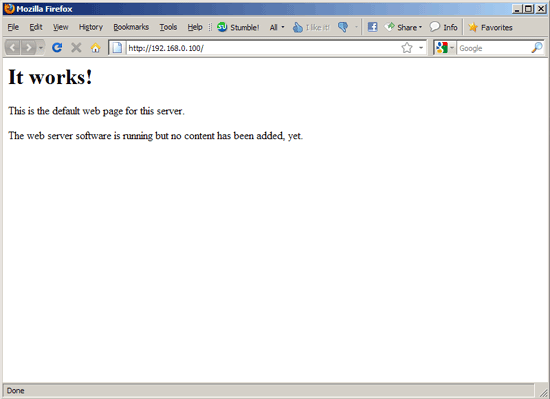
\includegraphics{apache2.png}

\item {} 
Install PHP5

PHP5 and the Apache PHP5 module are required to serve the EARS web-based
code.  Install them as follows:

\begin{Verbatim}[commandchars=\\\{\},formatcom=\footnotesize]
\PYGZpc{} aptitude install php5 libapache2-mod-php5
\end{Verbatim}

Restart Apache:

\begin{Verbatim}[commandchars=\\\{\},formatcom=\footnotesize]
\PYGZpc{} /etc/init.d/apache2 restart
\end{Verbatim}

\item {} 
Install MySQL support in PHP5

To get MySQL support in PHP, we can install the \emph{php5-mysql} package. It's
a good idea to install some other PHP5 modules as well as you might need
them for your applications.

\begin{Verbatim}[commandchars=\\\{\},formatcom=\footnotesize]
\PYGZpc{} aptitude install php5-mysql php5-curl php-pear php5-imagick \PYG{l+s+se}{\PYGZbs{}}
   php5-mcrypt php5-memcache
\end{Verbatim}

\begin{notice}{note}{Note:}
You can search for available PHP5 modules like
this:

\begin{Verbatim}[commandchars=\\\{\},formatcom=\footnotesize]
\PYGZpc{} apt-cache search php5
\end{Verbatim}
\end{notice}

Now restart Apache2:

\begin{Verbatim}[commandchars=\\\{\},formatcom=\footnotesize]
\PYGZpc{} /etc/init.d/apache2 restart
\end{Verbatim}

\end{enumerate}


\subsection{Git Installation}
\label{installation:git-installation}
\href{http://git-scm.com}{Git} \footnote{
\href{http://git-scm.com/book}{Pro Git} by Scott Chacon is available to read online for free.
} is required to download the EARS Milter code from the development
repository.
\begin{enumerate}
\item {} 
Install Git

\begin{Verbatim}[commandchars=\\\{\},formatcom=\footnotesize]
\PYGZpc{} aptitude install git
\end{Verbatim}

\item {} 
Configure git access
\begin{itemize}
\item {} 
On the EARS Milter server, create a \emph{ssh} key and copy it to the
development repository server:
\begin{quote}

\begin{Verbatim}[commandchars=\\\{\},formatcom=\footnotesize]
\PYGZpc{} ssh-keygen -t rsa
\end{Verbatim}

Hit return at the prompts to create the key without passphrase
authentication.

\begin{Verbatim}[commandchars=\\\{\},formatcom=\footnotesize]
\PYGZpc{} scp \PYGZti{}/.ssh/id\PYGZus{}rsa.pub root@git:/root
\end{Verbatim}
\end{quote}

\item {} 
Log in to the repository server and authorize the key:
\begin{quote}

\begin{Verbatim}[commandchars=\\\{\},formatcom=\footnotesize]
\PYGZpc{} ssh root@git
\PYGZpc{} \PYG{n+nb}{cd }gitolite-admin
\PYGZpc{} git pull
\PYGZpc{} cp \PYGZti{}/id\PYGZus{}rsa.pub keydir/root\PYG{l+s+se}{\PYGZbs{}@}\PYGZlt{}milterservername\PYGZgt{}.pub
\PYGZpc{} sed -i \PYG{l+s+s1}{'s/\PYGZbs{}@.*\PYGZdl{}//g'} keydir/root\PYG{l+s+se}{\PYGZbs{}@}\PYGZlt{}milterservername\PYGZgt{}.pub
\PYGZpc{} git add keydir/root\PYG{l+s+se}{\PYGZbs{}@}\PYGZlt{}milterservername\PYGZgt{}.pub
\PYGZpc{} git commit -a
\PYGZpc{} git push
\PYGZpc{} \PYG{n+nb}{exit}
\end{Verbatim}
\end{quote}

\item {} 
On the EARS Milter server, test access to the repository server:
\begin{quote}

\begin{Verbatim}[commandchars=\\\{\},formatcom=\footnotesize]
\PYGZpc{} \PYG{n+nb}{cd} /tmp
\PYGZpc{} git clone gitolite@git:gitolite-admin
\end{Verbatim}

If this fails, please verify all the steps in this section
\end{quote}

\end{itemize}

\end{enumerate}


\subsection{Mail Server Installation}
\label{installation:mail-server-installation}
EARS requires an MTA.  Please choose \textbf{either} postfix or sendmail.
\setbox0\vbox{
\begin{minipage}{0.95\linewidth}
\begin{itemize}
\item {} 
{\hyperref[installation:postfix-option-1]{Postfix (Option 1)}}

\item {} 
{\hyperref[installation:sendmail-option-2]{Sendmail (Option 2)}}

\end{itemize}
\end{minipage}}
\begin{center}\setlength{\fboxsep}{5pt}\shadowbox{\box0}\end{center}


\subsubsection{Postfix (Option 1)}
\label{installation:postfix-option-1}\begin{enumerate}
\item {} 
Install postfix with \href{http://www.pcre.org}{PCRE} support:

\begin{Verbatim}[commandchars=\\\{\},formatcom=\footnotesize]
\PYGZpc{} aptitude install postfix postfix-pcre
\end{Verbatim}

If prompted to remove packages relating to \code{exim4} or \code{sendmail},
choose to \emph{Accept the solution}.

When prompted for \emph{mail server configuration type}, choose
\emph{Satellite System}:

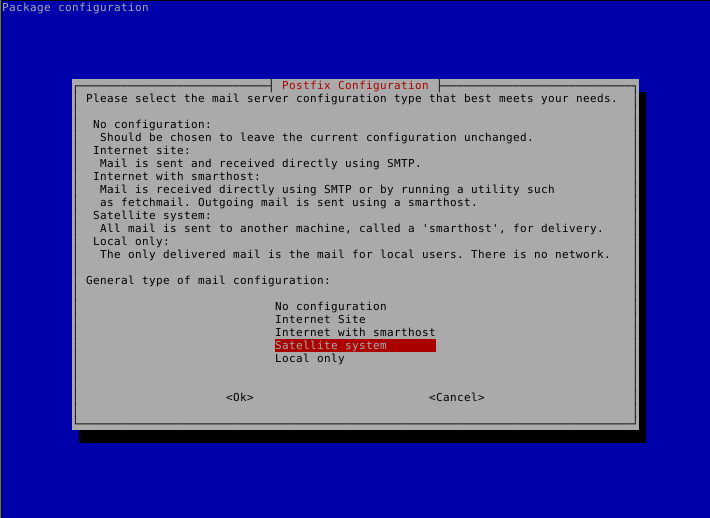
\includegraphics{postfix1.png}

Enter a fully-qualified domain name in the form of
\emph{servername.wrtdesign.com}, where \emph{servername} is the name of the EARS
Milter server. Make sure that there is a DNS entry for this server and its
corresponding IP address on the DNS server.

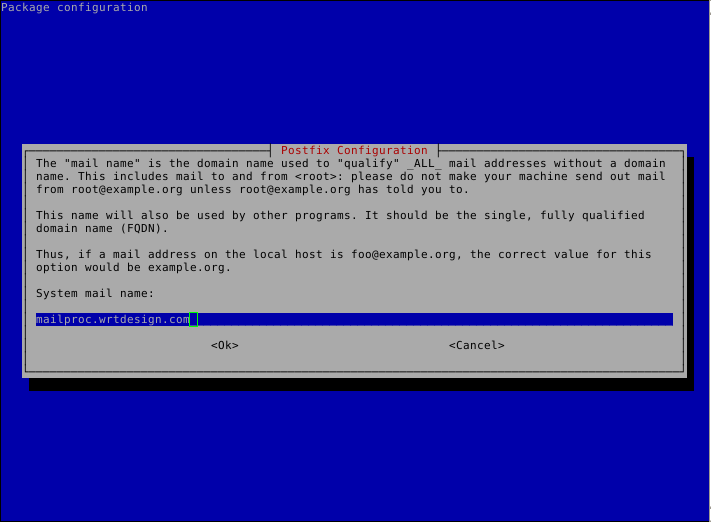
\includegraphics{postfix2.png}

Enter the FQDN of the MS Exchange server when prompted for a relay host:

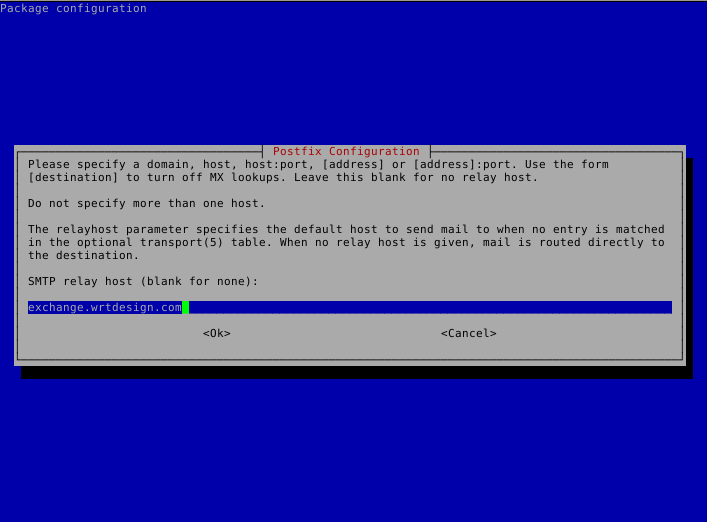
\includegraphics{postfix3.png}

Accept the defaults for \emph{Root and postmaster mail recipient},
\emph{Other destinations to accept mail for} and \emph{Force synchronous updates...}.

For \emph{Local networks}, enter \code{10.102.0.0/16, 192.168.0.0/24, 127.0.0.1}.
This will handle all of WRT's internal networks as well as the localhost.

Accept all the rest of the defaults.

\item {} 
Add the following lines to \code{/etc/postfix/main.cf}:

\begin{Verbatim}[commandchars=\\\{\},formatcom=\footnotesize]
\PYG{n+nv}{disable\PYGZus{}vrfy\PYGZus{}command} \PYG{o}{=} yes
\PYG{n+nv}{smtpd\PYGZus{}command\PYGZus{}filter} \PYG{o}{=} pcre:/etc/postfix/bogus\PYGZus{}commands
\PYG{n+nv}{smtpd\PYGZus{}recipient\PYGZus{}restrictions} \PYG{o}{=} permit\PYGZus{}mynetworks reject\PYGZus{}unauth\PYGZus{}destination
\end{Verbatim}

Remove the following line from the same file:

\begin{Verbatim}[commandchars=\\\{\},formatcom=\footnotesize]
\PYG{c}{\PYGZsh{}inet\PYGZus{}interfaces = loopback-only}
\end{Verbatim}

Edit the following line to read:

\begin{Verbatim}[commandchars=\\\{\},formatcom=\footnotesize]
\PYG{n+nv}{inet\PYGZus{}protocols} \PYG{o}{=} ipv4
\end{Verbatim}

\item {} 
Open up \code{/etc/postfix/master.cf} and uncomment the line:

\begin{Verbatim}[commandchars=\\\{\},formatcom=\footnotesize]
\PYG{c}{\PYGZsh{}submission inet n       -       -       -       -       smtpd}
\end{Verbatim}

Add the following lines (with indentation) to the same file:

\begin{Verbatim}[commandchars=\\\{\},formatcom=\footnotesize]
scan      unix  -       -       n       -       10      smtp
 -o \PYG{n+nv}{smtp\PYGZus{}send\PYGZus{}xforward\PYGZus{}command}\PYG{o}{=}yes
 -o \PYG{n+nv}{disable\PYGZus{}mime\PYGZus{}output\PYGZus{}conversion}\PYG{o}{=}yes
 -o \PYG{n+nv}{smtp\PYGZus{}generic\PYGZus{}maps}\PYG{o}{=}
\end{Verbatim}

Add the following (indented) after the line marked \code{relay}:

\begin{Verbatim}[commandchars=\\\{\},formatcom=\footnotesize]
-o \PYG{n+nv}{smtp\PYGZus{}fallback\PYGZus{}relay}\PYG{o}{=}
\end{Verbatim}

Change the follwing lines:

\begin{Verbatim}[commandchars=\\\{\},formatcom=\footnotesize]
-smtp      inet  n       -       -       -       -       smtpd
-cleanup   unix  n       -       -       -       0       cleanup
\end{Verbatim}

to read:

\begin{Verbatim}[commandchars=\\\{\},formatcom=\footnotesize]
-smtp      inet  n       -       n      -       -       smtpd
-cleanup   unix  n       -       n       -       0       cleanup
\end{Verbatim}

\item {} 
Create a file called \code{/etc/postfix/bogus\_commands} and enter the
following two lines:

\begin{Verbatim}[commandchars=\\\{\},formatcom=\footnotesize]
/\PYGZca{}\PYG{o}{[}\PYGZca{} \PYG{o}{]}\PYG{o}{\PYGZob{}}3\PYG{o}{\PYGZcb{}}\PYG{l+s+se}{\PYGZbs{}s}.*/  NOOP
/\PYGZca{}https\PYG{o}{\PYGZob{}}0,1\PYG{o}{\PYGZcb{}}\PYG{l+s+se}{\PYGZbs{}:}\PYG{l+s+se}{\PYGZbs{}/}\PYG{l+s+se}{\PYGZbs{}/}.*/ NOOP
\end{Verbatim}

\item {} 
Reload the configuration and send a test message:

\begin{Verbatim}[commandchars=\\\{\},formatcom=\footnotesize]
\PYGZpc{} postfix reload
\PYGZpc{} telnet localhost 25
telnet localhost 25
Trying 127.0.0.1...
Connected to localhost.
Escape character is \PYG{l+s+s1}{'\PYGZca{}]'}.
220 ph-wks-lin01.wrtdesign.com ESMTP Postfix \PYG{o}{(}Debian/GNU\PYG{o}{)}
ehlo localhost
250-ph-wks-lin01.wrtdesign.com
250-PIPELINING
250-SIZE 10240000
250-ETRN
250-STARTTLS
250-ENHANCEDSTATUSCODES
250-8BITMIME
250 DSN
mail from: root
250 2.1.0 Ok
rcpt to: ph\PYGZus{}test@wrtdesign.com
250 2.1.5 Ok
data
354 End data with \PYGZlt{}CR\PYGZgt{}\PYGZlt{}LF\PYGZgt{}.\PYGZlt{}CR\PYGZgt{}\PYGZlt{}LF\PYGZgt{}
\PYG{n+nb}{test}
.
250 2.0.0 Ok: queued as 4F00049F2A
quit
\end{Verbatim}

\end{enumerate}


\subsubsection{Sendmail (Option 2)}
\label{installation:sendmail-option-2}\begin{enumerate}
\item {} 
Install sendmail:

\begin{Verbatim}[commandchars=\\\{\},formatcom=\footnotesize]
\PYGZpc{} aptitude install sendmail
\end{Verbatim}

If prompted to remove packages relating to \code{exim4} or \code{postfix},
choose to \emph{Accept the solution}.

\item {} 
Open the file \code{/etc/mail/sendmail.mc} in an editor.  Add the following
lines above \code{MAILER DEFINITIONS}:

\begin{Verbatim}[commandchars=\\\{\},formatcom=\footnotesize]
dnl \PYG{c}{\PYGZsh{} FEATURE({}`allmasquerade')dnl FEATURE({}`masquerade\PYGZus{}envelope')dnl}
FEATURE\PYG{o}{(}\PYG{l+s+sb}{{}`}accept\PYGZus{}unresolvable\PYGZus{}domains\PYG{l+s+s1}{') FEATURE({}`accept\PYGZus{}unqualified\PYGZus{}senders'}\PYG{o}{)}
define\PYG{o}{(}\PYG{l+s+sb}{{}`}SMART\PYGZus{}HOST\PYG{l+s+s1}{',{}`exchange.domain.com'}\PYG{o}{)}dnl
define\PYG{o}{(}\PYG{l+s+sb}{{}`}confDOMAIN\PYGZus{}NAME\PYG{l+s+s1}{',{}`milterserver.domain.com'}\PYG{o}{)} dnl \PYG{c}{\PYGZsh{}}
\end{Verbatim}

Change these lines:

\begin{Verbatim}[commandchars=\\\{\},formatcom=\footnotesize]
dnl
DAEMON\PYGZus{}OPTIONS\PYG{o}{(}\PYG{l+s+sb}{{}`}\PYG{n+nv}{Family}\PYG{o}{=}inet6, \PYG{n+nv}{Name}\PYG{o}{=}MTA-v6, \PYG{n+nv}{Port}\PYG{o}{=}smtp, \PYG{n+nv}{Addr}\PYG{o}{=}::1\PYG{l+s+s1}{')dnl}
\PYG{l+s+s1}{DAEMON\PYGZus{}OPTIONS({}`Name=MTA-v4,Address=127.0.0.1,Family=inet,Port=smtp'}\PYG{o}{)}
dnl
DAEMON\PYGZus{}OPTIONS\PYG{o}{(}\PYG{l+s+sb}{{}`}\PYG{n+nv}{Family}\PYG{o}{=}inet6, \PYG{n+nv}{Name}\PYG{o}{=}MSP-v6, \PYG{n+nv}{Port}\PYG{o}{=}submission, \PYG{n+nv}{M}\PYG{o}{=}Ea, \PYG{n+nv}{Addr}\PYG{o}{=}::1\PYG{l+s+s1}{')dnl}
\PYG{l+s+s1}{DAEMON\PYGZus{}OPTIONS({}`Name=MSP-v4,Address=127.0.0.1,Family=inet,Port=submission,Modifiers=aE'}\PYG{o}{)}
\end{Verbatim}

to

\begin{Verbatim}[commandchars=\\\{\},formatcom=\footnotesize]
dnl
DAEMON\PYGZus{}OPTIONS\PYG{o}{(}\PYG{l+s+sb}{{}`}\PYG{n+nv}{Family}\PYG{o}{=}inet6, \PYG{n+nv}{Name}\PYG{o}{=}MTA-v6, \PYG{n+nv}{Port}\PYG{o}{=}smtp, \PYG{n+nv}{Addr}\PYG{o}{=}::1\PYG{l+s+s1}{')dnl}
\PYG{l+s+s1}{DAEMON\PYGZus{}OPTIONS({}`Name=MTA,Family=inet,Port=smtp'}\PYG{o}{)}
dnl
DAEMON\PYGZus{}OPTIONS\PYG{o}{(}\PYG{l+s+sb}{{}`}\PYG{n+nv}{Family}\PYG{o}{=}inet6, \PYG{n+nv}{Name}\PYG{o}{=}MSP-v6, \PYG{n+nv}{Port}\PYG{o}{=}submission, \PYG{n+nv}{M}\PYG{o}{=}Ea, \PYG{n+nv}{Addr}\PYG{o}{=}::1\PYG{l+s+s1}{')dnl}
\PYG{l+s+s1}{DAEMON\PYGZus{}OPTIONS({}`Name=MSP,Family=inet,Port=submission,Modifiers=aE'}\PYG{o}{)}
\end{Verbatim}

\item {} 
Open the file \code{/etc/mail/access}.  Uncomment the following lines
(according to your network):

\begin{Verbatim}[commandchars=\\\{\},formatcom=\footnotesize]
Connect:10
RELAY GreetPause:10           0
ClientConn:10           OK
ClientRate:10           0
\end{Verbatim}

Add additional lines for each FQDN of this IP address

\item {} 
Add all internal recipient domains to \code{/etc/mail/relay-domains}

Example:
\begin{quote}

\begin{Verbatim}[commandchars=\\\{\},formatcom=\footnotesize]
wrtdesign.com ph.wrtdesign.com
\end{Verbatim}
\end{quote}

\item {} 
Recompile the \code{sendmail} files and restart the MTA and send a test
message

\begin{Verbatim}[commandchars=\\\{\},formatcom=\footnotesize]
\PYGZpc{} touch /etc/mail/access.new.db
\PYGZpc{} sendmailconfig
\PYGZpc{} telnet localhost 25
Connected to localhost.
Escape character is \PYG{l+s+s1}{'\PYGZca{}]'}.
220 mailproc-test2 ESMTP
ehlo localhost
250-mailproc-test2 Hello localhost \PYG{o}{[}127.0.0.1\PYG{o}{]}, pleased to meet you
250-ENHANCEDSTATUSCODES
250-PIPELINING
250-EXPN
250-VERB
250-8BITMIME
250-SIZE
250-DSN
250-ETRN
250-DELIVERBY
250 HELP
mail from: root
250 2.1.0 root... Sender ok
rcpt to: ph\PYGZus{}test@wrtdesign.com
250 2.1.5 ph\PYGZus{}test@wrtdesign.com... Recipient ok
data
354 Enter mail, end with \PYG{l+s+s2}{"."} on a line by itself
\PYG{n+nb}{test}
.
250 2.0.0 q7VDE019017465 Message accepted \PYG{k}{for }delivery
quit
\end{Verbatim}

\end{enumerate}


\section{Python Installation/Configuration}
\label{installation:python-installation-configuration}\setbox0\vbox{
\begin{minipage}{0.95\linewidth}
\begin{itemize}
\item {} 
{\hyperref[installation:the-python-method-preferred]{The Python Method (preferred)}}

\item {} 
{\hyperref[installation:the-debian-method]{The Debian Method}}

\end{itemize}
\end{minipage}}
\begin{center}\setlength{\fboxsep}{5pt}\shadowbox{\box0}\end{center}

The default version of Python in Debian Squeeze/Wheezy is 2.7.  This is what we
will be installing, along with a Python package installer (pip) and some
development libraries.

\begin{Verbatim}[commandchars=\\\{\},formatcom=\footnotesize]
\PYGZpc{} aptitude install python python-pip python-dev libmilter-dev libmilter1.0.1  libmysqlclient-dev
\end{Verbatim}

Next we will need to install a number of Python modules.  There are two ways to
do this - the Debian way and the Python way. Each one has its advantages and
disadvantages, but both are provided for instructional purposes.

The recommendation is to stick with one method instead of combining them.


\subsection{The Python Method (preferred)}
\label{installation:the-python-method-preferred}
The Python Package Index (\href{http://pypi.python.org}{PyPI}) is the most up-to-date resource for Python
modules.  Bugfixes and updates are regularly submitted for a majority of
modules.  The downside is that there is currenlty no way to automatically
update the modules, but this can be considered a benefit as well since there is
less chance of your code breaking.

\begin{Verbatim}[commandchars=\\\{\},formatcom=\footnotesize]
\PYGZpc{} pip install SQLAlchemy pymilter MySQL-python Mako tnefparse dnspython
\end{Verbatim}


\subsection{The Debian Method}
\label{installation:the-debian-method}
Using debian's built-in package manager is very easy and convenient.  When you
do a full update on a Debian system, installed Python modules will be updated
as well.  The downside is that sometimes the modules in the Debian repositories
can be out-of-date.

Here is the simple command to install the required modules, except for
\code{tnefparse} which has to be installed via the Python method:

\begin{Verbatim}[commandchars=\\\{\},formatcom=\footnotesize]
\PYGZpc{} aptitude install python-sqlalchemy python-milter python-mysqldb python-mako
\end{Verbatim}


\section{Optional Software Installation}
\label{installation:optional-software-installation}\setbox0\vbox{
\begin{minipage}{0.95\linewidth}
\begin{itemize}
\item {} 
{\hyperref[installation:phpmyadmin]{phpMyAdmin}}

\item {} 
{\hyperref[installation:webmin-installation]{Webmin Installation}}

\end{itemize}
\end{minipage}}
\begin{center}\setlength{\fboxsep}{5pt}\shadowbox{\box0}\end{center}


\subsection{phpMyAdmin}
\label{installation:phpmyadmin}
\href{http://www.phpmyadmin.net}{phpMyAdmin} is a web interface through which you can manage your MySQL
databases. It's a good idea to install it:

\begin{Verbatim}[commandchars=\\\{\},formatcom=\footnotesize]
\PYGZpc{} aptitude install phpmyadmin php5-gd
\end{Verbatim}

You will see the following question:
\begin{quote}

\begin{DUlineblock}{0em}
\item[] \code{Web server to reconfigure automatically:} \textless{}-- apache2
\item[] \code{Configure database for phpmyadmin with dbconfig-common?} \textless{}-- No
\end{DUlineblock}
\end{quote}

Afterwards, you can access phpMyAdmin by going to
\code{http://\textless{}serverIP\textgreater{}/phpmyadmin/:}

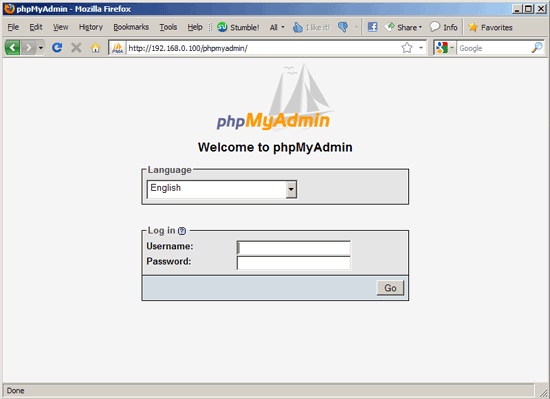
\includegraphics{phpMyAdmin.png}


\subsection{Webmin Installation}
\label{installation:webmin-installation}\begin{enumerate}
\item {} 
Create a file called \code{/etc/apt/sources.list.d/webmin.list}.  Add the
following lines, then save:

\begin{Verbatim}[commandchars=\\\{\},formatcom=\footnotesize]
deb http://download.webmin.com/download/repository sarge contrib
deb http://webmin.mirror.somersettechsolutions.co.uk/repository sarge contrib
\end{Verbatim}

\item {} 
Download and install the security key, then update and install \code{webmin}:

\begin{Verbatim}[commandchars=\\\{\},formatcom=\footnotesize]
\PYGZpc{} \PYG{n+nb}{cd} /root
\PYGZpc{} wget http://www.webmin.com/jcameron-key.asc
\PYGZpc{} apt-key add jcameron-key.asc
\PYGZpc{} aptitude update
\PYGZpc{} aptitude install webmin
\end{Verbatim}

\item {} 
Test the installation by going to \code{https://\textless{}serverIP\textgreater{}:10000}.  Log in
using the system root password.

\end{enumerate}


\section{Accquiring and configuring the Milter}
\label{installation:accquiring-and-configuring-the-milter}\begin{enumerate}
\item {} 
Using \emph{git}, clone \textbf{EARS} from the repository to the \code{/var/spool}
folder:

\begin{Verbatim}[commandchars=\\\{\},formatcom=\footnotesize]
\PYGZpc{} \PYG{n+nb}{cd} /var/spool
\PYGZpc{} git clone gitolite@git:EARSmilter EARS
\PYGZpc{} \PYG{n+nb}{cd }EARS
\end{Verbatim}

\item {} 
Copy EARS.sh to \code{/etc/init.d}.  Make it executable and enable it
at boot.

\begin{Verbatim}[commandchars=\\\{\},formatcom=\footnotesize]
\PYGZpc{} cp /var/spool/EARS/EARS.sh /etc/init.d
\PYGZpc{} chmod +x /etc/init.d/EARS.sh
\PYGZpc{} update-rc.d EARS.sh \PYG{n+nb}{enable }defaults
\end{Verbatim}

\item {} 
Create a virtual host file for Apache in
\code{/etc/apache2/sites-available/ears.conf} that contains the following
(modify as necessary):

\begin{Verbatim}[commandchars=\\\{\},formatcom=\footnotesize]
\PYGZlt{}VirtualHost *:80\PYGZgt{}
   ServerName ears.wrtdesign.com
   DocumentRoot /var/www/EARS
   Options -Indexes
\PYGZlt{}/VirtualHost\PYGZgt{}
\end{Verbatim}

Create a link to this file to make the site active:

\begin{Verbatim}[commandchars=\\\{\},formatcom=\footnotesize]
\PYGZpc{} ln -s /etc/apache2/sites-available/ears.conf \PYG{l+s+se}{\PYGZbs{}}
/etc/apache2/sites-enabled/ears.conf
\end{Verbatim}

Create a folder called \code{/var/www/EARS}.  Copy the files from
\code{/var/spool/EARS/www} to this new folder and give Apache full rights to
the folder. Restart Apache.

\begin{Verbatim}[commandchars=\\\{\},formatcom=\footnotesize]
\PYGZpc{} mkdir -p /var/www/EARS
\PYGZpc{} cp -R /var/spool/EARS/www/* /var/www/EARS
\PYGZpc{} chown -R www-data.www-data  /var/www/EARS
\PYGZpc{} chmod -x /var/www/EARS/*.php
\PYGZpc{} /etc/init.d/apache2 restart
\end{Verbatim}

\item {} 
Open the MySQL command-line utility

\begin{Verbatim}[commandchars=\\\{\},formatcom=\footnotesize]
\PYGZpc{} mysql -u \PYG{l+s+s1}{'root'} -p
\end{Verbatim}

Create a blank database and associated MySQL user

\begin{Verbatim}[commandchars=\\\{\},formatcom=\footnotesize]
\PYG{n}{mysql}\PYG{o}{\PYGZgt{}} \PYG{k}{CREATE} \PYG{k}{DATABASE} \PYG{n}{EARS}\PYG{p}{;}
\PYG{n}{mysql}\PYG{o}{\PYGZgt{}} \PYG{k}{GRANT} \PYG{k}{ALL} \PYG{k}{PRIVILEGES} \PYG{k}{ON} \PYG{n}{EARS}\PYG{p}{.}\PYG{o}{*} \PYG{k}{TO} \PYG{l+s+ss}{"EARS"}\PYG{o}{@}\PYG{l+s+ss}{"\PYGZpc{}"} \PYG{n}{IDENTIFIED} \PYG{k}{BY} \PYG{l+s+ss}{"password"}\PYG{p}{;}
\PYG{n}{mysql}\PYG{o}{\PYGZgt{}} \PYG{n}{FLUSH} \PYG{k}{PRIVILEGES}\PYG{p}{;} \PYG{n}{mysql}\PYG{o}{\PYGZgt{}} \PYG{n}{EXIT}
\end{Verbatim}

and change this line in \code{/etc/mysql/my.cnf}:

\begin{Verbatim}[commandchars=\\\{\},formatcom=\footnotesize]
\PYG{n+nb}{bind}-address \PYG{o}{=} 127.0.0.1
\end{Verbatim}

to:

\begin{Verbatim}[commandchars=\\\{\},formatcom=\footnotesize]
\PYG{n+nb}{bind}-address \PYG{o}{=} 0.0.0.0
\end{Verbatim}

\item {} 
Set the appropriate permissions on \code{/var/spool/EARS} and its
subdirectories based on the MTA installed.

Postfix

\begin{Verbatim}[commandchars=\\\{\},formatcom=\footnotesize]
\PYGZpc{} chown -R postfix.postfix /var/spool/EARS
\end{Verbatim}

Sendmail

\begin{Verbatim}[commandchars=\\\{\},formatcom=\footnotesize]
\PYGZpc{} chown -R smmta.smmta /var/spool/EARS
\end{Verbatim}

You will also need to edit \code{/etc/init.d/EARS.sh} and replace \textbf{postfix}
with \textbf{smmta}.

\begin{Verbatim}[commandchars=\\\{\},formatcom=\footnotesize]
\PYGZpc{} sed -i.bak \PYG{l+s+s1}{'s/postfix/smmta/g'} /etc/init.d/EARS.sh
\end{Verbatim}

\item {} 
Create the log files:

\begin{Verbatim}[commandchars=\\\{\},formatcom=\footnotesize]
\PYGZpc{} touch /var/log/EARSmilter.log
\PYGZpc{} touch /var/log/EARSmilter.err
\PYGZpc{} chmod 666 /var/log/EARSmilter.log
\PYGZpc{} chmod 666 /var/log/EARSmilter.err
\end{Verbatim}

\item {} 
Add/edit the following lines to the configuration file for the appropriate
MTA:

\textbf{Postfix} - \code{/etc/postfix/main.cf}

\begin{Verbatim}[commandchars=\\\{\},formatcom=\footnotesize]
\PYG{n+nv}{milter\PYGZus{}protocol} \PYG{o}{=} 6
\PYG{n+nv}{smtpd\PYGZus{}milters} \PYG{o}{=} unix:/var/spool/EARS/EARSmilter.sock
\PYG{n+nv}{milter\PYGZus{}default\PYGZus{}action} \PYG{o}{=} accept
\end{Verbatim}

Reload postfix

\begin{Verbatim}[commandchars=\\\{\},formatcom=\footnotesize]
\PYGZpc{} postfix reload
\end{Verbatim}

\end{enumerate}
\begin{quote}

\textbf{Sendmail} - \code{/etc/mail/sendmail.mc}.
\begin{quote}

\begin{Verbatim}[commandchars=\\\{\},formatcom=\footnotesize]
INPUT\PYGZus{}MAIL\PYGZus{}FILTER\PYG{o}{(}\PYG{l+s+sb}{{}`}EARS\PYG{l+s+s1}{', {}`S=unix:/var/spool/EARS/EARSmilter.sock, F=T, T=S:240s;R:240s;E:5m'}\PYG{o}{)}dnl
\end{Verbatim}

Recompile the \code{sendmail} files and restart the MTA

\begin{Verbatim}[commandchars=\\\{\},formatcom=\footnotesize]
\PYGZpc{} touch /etc/mail/access.new.db
\PYGZpc{} sendmailconfig
\end{Verbatim}

\begin{notice}{note}{Note:}
If/when you add additional milters to this sytem, make sure that
\textbf{EARS} is the last one listed, as milters are processed in order.
\end{notice}
\end{quote}
\end{quote}
\begin{enumerate}
\item {} 
Edit the database information in
\code{/var/spool/EARS/EARSmilter/EARSmilter.py} with what is appropriate for
your environment.

This is listed under \code{EARSmilter.EARSmilter.milter.eom()}

\begin{Verbatim}[commandchars=\\\{\},formatcom=\footnotesize]
\PYG{n}{db} \PYG{o}{=} \PYG{n}{toDB}\PYG{p}{(} \PYG{l+s}{'}\PYG{l+s}{username}\PYG{l+s}{'}\PYG{p}{,} \PYG{l+s}{'}\PYG{l+s}{password}\PYG{l+s}{'}\PYG{p}{,} \PYG{l+s}{'}\PYG{l+s}{MySQLServer}\PYG{l+s}{'}\PYG{p}{,} \PYG{l+s}{'}\PYG{l+s}{EARSDataBase}\PYG{l+s}{'} \PYG{p}{)}
\end{Verbatim}

\item {} 
Create a folder called \code{/dropdir} :

\begin{Verbatim}[commandchars=\\\{\},formatcom=\footnotesize]
\PYGZpc{} mkdir -p /dropdir
\end{Verbatim}

Mount it to a folder called \code{dropdir} on a FTP server.  This example
assumes the folder is on a MS Windows box:

\begin{Verbatim}[commandchars=\\\{\},formatcom=\footnotesize]
\PYGZpc{} \PYG{n+nb}{echo} \PYG{l+s+s1}{'\PYGZbs{}\PYGZbs{}FTPSERVER\PYGZbs{}FTPSHARE\PYGZbs{}dropdir  /dropdir  cifs  workgroup=DOMAIN, \PYGZbs{}}
\PYG{l+s+s1}{   file\PYGZus{}mode=0777,dir\PYGZus{}mode=0777,password=PASSWORD,uid=1000,gid=1000, \PYGZbs{}}
\PYG{l+s+s1}{   username=USERNAME 0  0'} \PYGZgt{}\PYGZgt{} /etc/fstab
\PYGZpc{} mount -a
\end{Verbatim}

\item {} 
Start the EARS milter:

\begin{Verbatim}[commandchars=\\\{\},formatcom=\footnotesize]
/etc/init.d/EARS.sh start
\end{Verbatim}

\item {} 
Add a \code{cron} job to run the \code{purgeEARSdb} script on a weekly basis.

\begin{Verbatim}[commandchars=\\\{\},formatcom=\footnotesize]
\PYGZpc{} crontab -e
\end{Verbatim}

\end{enumerate}
\begin{quote}

Add this line:

\begin{Verbatim}[commandchars=\\\{\},formatcom=\footnotesize]
@daily /usr/bin/env python /var/spool/EARS/purgeEARSdb/purgeEARSdb.py -s \PYG{l+s+se}{\PYGZbs{}}
   milter.domain.com -d EARS -u EARS -p password -q -x -v\PYGZsh{}purge EARS database
\end{Verbatim}

For a description of the options, see \textbf{How To Use} under {\hyperref[codedocs/purgeEARSdb_py:module-purgeEARSdb]{\code{purgeEARSdb()}}}.
\end{quote}
\begin{enumerate}
\item {} 
Add the following lines to \code{/etc/logrotate.conf}:

\begin{Verbatim}[commandchars=\\\{\},formatcom=\footnotesize]
/var/log/EARSmilter.* \PYG{o}{\PYGZob{}}
  compress copytruncate
\PYG{o}{\PYGZcb{}}
\end{Verbatim}

\end{enumerate}


\chapter{EARS Code}
\label{codedocs:how-to-use}\label{codedocs:ears-code}\label{codedocs::doc}

\section{EARS.py}
\label{codedocs/EARS_py:ears-py}\label{codedocs/EARS_py::doc}\label{codedocs/EARS_py:module-EARS}\index{EARS (module)}

\section{EARS Milter main class/functions}
\label{codedocs/EARSmilter:module-EARSmilter}\label{codedocs/EARSmilter:ears-milter-main-class-functions}\label{codedocs/EARSmilter::doc}\index{EARSmilter (module)}\begin{itemize}
\item {} 
{\hyperref[codedocs/EARSmilter:earslog]{\emph{EARSlog}}}

\item {} 
{\hyperref[codedocs/EARSmilter:milter]{\emph{milter}}}

\item {} 
{\hyperref[codedocs/EARSmilter:processmessage]{\emph{ProcessMessage}}}

\item {} 
{\hyperref[codedocs/EARSmilter:filesys]{\emph{FileSys}}}

\end{itemize}


\subsection{EARSlog}
\label{codedocs/EARSmilter:earslog}\label{codedocs/EARSmilter:id1}\index{EARSlog (class in EARSmilter.EARSmilter)}

\begin{fulllineitems}
\phantomsection\label{codedocs/EARSmilter:EARSmilter.EARSmilter.EARSlog}\pysigline{\strong{class }\code{EARSmilter.EARSmilter.}\bfcode{EARSlog}}
\end{fulllineitems}



\subsection{milter}
\label{codedocs/EARSmilter:milter}\label{codedocs/EARSmilter:id2}\index{milter (class in EARSmilter.EARSmilter)}

\begin{fulllineitems}
\phantomsection\label{codedocs/EARSmilter:EARSmilter.EARSmilter.milter}\pysiglinewithargsret{\strong{class }\code{EARSmilter.EARSmilter.}\bfcode{milter}}{\emph{Milter.Base}}{}~\index{milter.connect() (in module EARSmilter)}

\begin{fulllineitems}
\pysigline{\bfcode{@Milter.noreply}}\phantomsection\label{codedocs/EARSmilter:EARSmilter.milter.connect}\pysiglinewithargsret{\bfcode{connect}}{\emph{IPname}, \emph{family}, \emph{hostaddr}}{}
Initializes when a new connection to the Milter is made via SMTP

\end{fulllineitems}

\index{milter.header() (in module EARSmilter)}

\begin{fulllineitems}
\pysigline{\bfcode{@Milter.noreply}}\phantomsection\label{codedocs/EARSmilter:EARSmilter.milter.header}\pysiglinewithargsret{\bfcode{header}}{\emph{name}, \emph{hval}}{}
Processes headers from the incoming message and writes them to a variable for database storage

\begin{Verbatim}[commandchars=\\\{\},formatcom=\footnotesize]
\PYG{n}{rgxSubject} \PYG{o}{=} \PYG{n}{re}\PYG{o}{.}\PYG{n}{compile}\PYG{p}{(} \PYG{l+s}{'}\PYG{l+s}{\PYGZca{}(subject)}\PYG{l+s}{'}\PYG{p}{,} \PYG{n}{re}\PYG{o}{.}\PYG{n}{IGNORECASE} \PYG{o}{\textbar{}} \PYG{n}{re}\PYG{o}{.}\PYG{n}{DOTALL} \PYG{p}{)}
\PYG{n}{rgxMessageID} \PYG{o}{=} \PYG{n}{re}\PYG{o}{.}\PYG{n}{compile}\PYG{p}{(} \PYG{l+s}{'}\PYG{l+s}{\PYGZca{}(message-id)}\PYG{l+s}{'}\PYG{p}{,} \PYG{n}{re}\PYG{o}{.}\PYG{n}{IGNORECASE} \PYG{o}{\textbar{}} \PYG{n}{re}\PYG{o}{.}\PYG{n}{DOTALL} \PYG{p}{)}
\end{Verbatim}

Regular Expression searches used to extract and log the Subject and Message ID of incoming messages

\end{fulllineitems}


\end{fulllineitems}



\subsection{ProcessMessage}
\label{codedocs/EARSmilter:processmessage}\label{codedocs/EARSmilter:id3}\index{ProcessMessage (class in EARSmilter.EARSmilter)}

\begin{fulllineitems}
\phantomsection\label{codedocs/EARSmilter:EARSmilter.EARSmilter.ProcessMessage}\pysiglinewithargsret{\strong{class }\code{EARSmilter.EARSmilter.}\bfcode{ProcessMessage}}{\emph{\_db}, \emph{\_log}, \emph{\_from}}{}
\end{fulllineitems}



\subsection{FileSys}
\label{codedocs/EARSmilter:id4}\label{codedocs/EARSmilter:filesys}\index{FileSys (class in EARSmilter.EARSmilter)}

\begin{fulllineitems}
\phantomsection\label{codedocs/EARSmilter:EARSmilter.EARSmilter.FileSys}\pysiglinewithargsret{\strong{class }\code{EARSmilter.EARSmilter.}\bfcode{FileSys}}{\emph{msg}}{}
\end{fulllineitems}



\section{purgeEARSdb.py}
\label{codedocs/purgeEARSdb_py:purgeearsdb-py}\label{codedocs/purgeEARSdb_py::doc}\label{codedocs/purgeEARSdb_py:module-purgeEARSdb}\index{purgeEARSdb (module)}
EARS Database Purge
\index{Options (class in purgeEARSdb.purgeEARSdb)}

\begin{fulllineitems}
\phantomsection\label{codedocs/purgeEARSdb_py:purgeEARSdb.purgeEARSdb.Options}\pysigline{\strong{class }\code{purgeEARSdb.purgeEARSdb.}\bfcode{Options}}
Establish the command-line options for purgeEARSdb.py

\begin{notice}{note}{Note:}
For command-line usage, see {\hyperref[codedocs/purgeEARSdb_py:how-to-use]{\emph{How to use}}}.
\end{notice}

\end{fulllineitems}

\index{Purge (class in purgeEARSdb.purgeEARSdb)}

\begin{fulllineitems}
\phantomsection\label{codedocs/purgeEARSdb_py:purgeEARSdb.purgeEARSdb.Purge}\pysiglinewithargsret{\strong{class }\code{purgeEARSdb.purgeEARSdb.}\bfcode{Purge}}{\emph{options}}{}~\index{purgeAttachmentsMessages() (purgeEARSdb.purgeEARSdb.Purge method)}

\begin{fulllineitems}
\phantomsection\label{codedocs/purgeEARSdb_py:purgeEARSdb.purgeEARSdb.Purge.purgeAttachmentsMessages}\pysiglinewithargsret{\bfcode{purgeAttachmentsMessages}}{}{}~
\begin{Verbatim}[commandchars=\\\{\},formatcom=\footnotesize]
\PYG{n}{query} \PYG{o}{=} \PYG{n}{session}\PYG{o}{.}\PYG{n}{query}\PYG{p}{(} \PYG{n}{Attachment} \PYG{p}{)}\PYG{o}{.}\PYG{n}{filter}\PYG{p}{(} \PYG{n}{Attachment}\PYG{o}{.}\PYG{n}{received} \PYG{o}{\PYGZlt{}}\PYG{o}{=} \PYG{n}{delta} \PYG{p}{)}\PYG{o}{.}\PYG{n}{all}\PYG{p}{(}\PYG{p}{)}
\end{Verbatim}

Searches attachments based on provided delta time (default of 7 days)

\begin{Verbatim}[commandchars=\\\{\},formatcom=\footnotesize]
\PYG{k}{for} \PYG{n}{q} \PYG{o+ow}{in} \PYG{n}{query}\PYG{p}{:}
    \PYG{k}{for} \PYG{n}{message} \PYG{o+ow}{in} \PYG{n}{q}\PYG{o}{.}\PYG{n}{message}\PYG{p}{:}
        \PYG{k}{if} \PYG{n}{message}\PYG{o}{.}\PYG{n}{dateReceived} \PYG{o}{\PYGZlt{}}\PYG{o}{=} \PYG{n}{delta}\PYG{p}{:}
\end{Verbatim}

Only deletes messages older than the specified delta.

\end{fulllineitems}

\index{purgeSenders() (purgeEARSdb.purgeEARSdb.Purge method)}

\begin{fulllineitems}
\phantomsection\label{codedocs/purgeEARSdb_py:purgeEARSdb.purgeEARSdb.Purge.purgeSenders}\pysiglinewithargsret{\bfcode{purgeSenders}}{}{}
Designed to remove senders with no assocated messages from the database

\end{fulllineitems}

\index{query\_yes\_no() (purgeEARSdb.purgeEARSdb.Purge method)}

\begin{fulllineitems}
\phantomsection\label{codedocs/purgeEARSdb_py:purgeEARSdb.purgeEARSdb.Purge.query_yes_no}\pysiglinewithargsret{\bfcode{query\_yes\_no}}{\emph{question}, \emph{default='yes'}}{}
Ask a yes/no question via raw\_input() and return their answer.

``question'' is a string that is presented to the user.
``default'' is the presumed answer if the user just hits \textless{}Enter\textgreater{}.
\begin{quote}

It must be ``yes'' (the default), ``no'' or None (meaning
an answer is required of the user).
\end{quote}

The ``answer'' return value is one of ``yes'' or ``no''.

\end{fulllineitems}


\end{fulllineitems}



\subsection{How to use}
\label{codedocs/purgeEARSdb_py:how-to-use}\label{codedocs/purgeEARSdb_py:id1}
Proper usage of purgeEARSdb.py

\begin{Verbatim}[commandchars=\\\{\},formatcom=\footnotesize]
usage: purgeEARSdb.py \PYG{o}{[}-h\PYG{o}{]} \PYG{o}{[}-q\PYG{o}{]} \PYG{o}{[}-v\PYG{o}{]} \PYG{o}{[}-D DAYS\PYG{o}{]} \PYG{o}{[}-H HOURS\PYG{o}{]} \PYG{o}{[}-M MINUTES\PYG{o}{]} \PYG{o}{[}-x\PYG{o}{]} -s
                   SERVER -d DATABASE -u USERNAME -p PASSWORD

Purge old messages/attachments from EARS database

optional arguments:
  -h, --help            show this \PYG{n+nb}{help }message and \PYG{n+nb}{exit}

 -q, --quiet           Run without prompting
  -v, --verbose         Verbose output

Message/Attachment age options:
  -D DAYS, --days DAYS  Remove message older than x days \PYG{o}{(}\PYG{n+nv}{default} \PYG{o}{=} 7\PYG{o}{)}
  -H HOURS, --hours HOURS
                        Remove message older than x hours \PYG{o}{(}\PYG{n+nv}{default} \PYG{o}{=} 0\PYG{o}{)}
  -M MINUTES, --minutes MINUTES
                        Remove message older than x minutes \PYG{o}{(}\PYG{n+nv}{default} \PYG{o}{=} 0\PYG{o}{)}

Sender Options:
  -x, --purge-senders   Purge senders from database that are no longer
                        associated with messages/attachments

Database Options \PYG{o}{(}required\PYG{o}{)}:
  -s SERVER, --server SERVER
                        MySQL server name
  -d DATABASE, --database DATABASE
                        MySQL database name
  -u USERNAME, --username USERNAME
                        MySQL username
  -p PASSWORD, --password PASSWORD
                        MySQL password
\end{Verbatim}

Example \textbf{cron} job setup:

\begin{Verbatim}[commandchars=\\\{\},formatcom=\footnotesize]
@daily /usr/bin/env python /var/spool/EARS/purgeEARSdb/purgeEARSdb.py -s mailproc.wrtdesign.com -d EARS -u EARS -p WRTears -q -x -v
\end{Verbatim}

This setups a daily job to run the script and remove non-associated senders from the database using the default of 7 days


\section{Database Definitions and Functions}
\label{codedocs/database:database-definitions-and-functions}\label{codedocs/database::doc}\phantomsection\label{codedocs/database:sqlalchemy}\phantomsection\label{codedocs/database:module-database.SQLAlchemy}\phantomsection\label{codedocs/database:sqlalchemy}\index{database.SQLAlchemy (module)}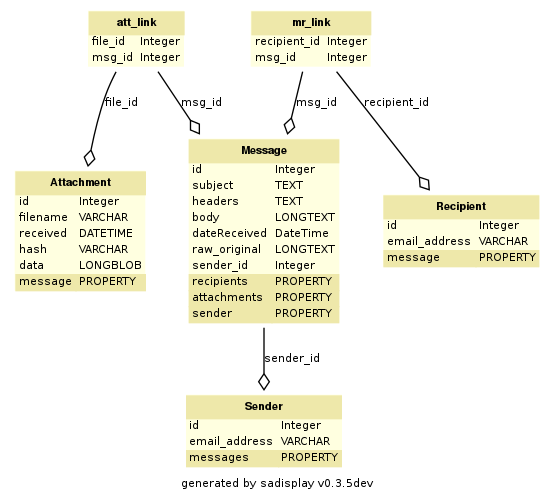
\includegraphics{sadisplay-6eaf309bd450fd536a3de386f2bd1c402f775f00.png}\phantomsection\label{codedocs/database:module-database.toDB}\index{database.toDB (module)}

\section{Customized Python Logging}
\label{codedocs/logs:customized-python-logging}\label{codedocs/logs::doc}\label{codedocs/logs:module-logs}\index{logs (module)}\phantomsection\label{codedocs/logs:module-logs.logger}\index{logs.logger (module)}
Created on Apr 23, 2012

@author: lwapnitsky


\chapter{Indices and tables}
\label{index:indices-and-tables}\begin{itemize}
\item {} 
\emph{genindex}

\item {} 
\emph{search}

\item {} 
\emph{modindex}

\end{itemize}



\renewcommand{\indexname}{Index}
\printindex
\end{document}
